\chapter{Validazione Funzionale}
\label{ch:validazione}

In questo capitolo viene descritta la validazione funzionale della piattaforma ChillChain attraverso uno scenario d'uso completo che attraversa tutte le funzionalità del sistema, coinvolgendo i tre ruoli previsti: amministratore, cliente e tecnico. Lo scenario simula un caso realistico in cui un'azienda di trasporti refrigerati gestisce una flotta di veicoli, riceve richieste di spedizione da più clienti e rileva un'anomalia sull'impianto frigorifero durante il viaggio.


% ============================================================================
\section{Ambiente di test}
\label{sec:ambiente_test}

La validazione è stata condotta su una macchina locale con l'intero sistema eseguito in container Docker. L'avvio avviene tramite un singolo comando \texttt{docker-compose up --build}, che istanzia i sei servizi descritti nel Capitolo~\ref{ch:soluzione}: il backend Spring Boot, il frontend React, il broker Mosquitto, il servizio di streaming Python, il servizio di anomaly detection e MongoDB. Dopo l'avvio, il frontend è raggiungibile all'indirizzo \texttt{http://localhost:5173} e il backend risponde sulla porta 8081.

Per la simulazione della telemetria sono stati predisposti dataset CSV generati dallo script di simulazione termodinamica descritto nella Sezione~\ref{sec:generazione_dati}: un dataset in condizioni di funzionamento normale per 120 minuti e un dataset con iniezione del guasto \texttt{UNDERCHARGE\_AND\_COND\_FOUL} (sottocaricamento del refrigerante combinato a fouling del condensatore) a partire dal minuto 60. Entrambi i dataset sono composti da 120 righe con campionamento al minuto.


% ============================================================================
\section{Scenario di validazione}
\label{sec:scenario}

Lo scenario è strutturato in cinque fasi che coprono l'intero ciclo di vita di una spedizione, dalla configurazione della flotta fino alla rilevazione di un'anomalia in corso di viaggio.


% ----------------------------------------------------------------------------
\subsection{Fase 1 --- Configurazione della flotta (Amministratore)}
\label{subsec:fase1}

L'amministratore accede alla piattaforma con le proprie credenziali e viene indirizzato alla dashboard di gestione della flotta. Da questa vista, procede alla registrazione di due veicoli refrigerati nella flotta.

\begin{figure}[ht]
\centering
% 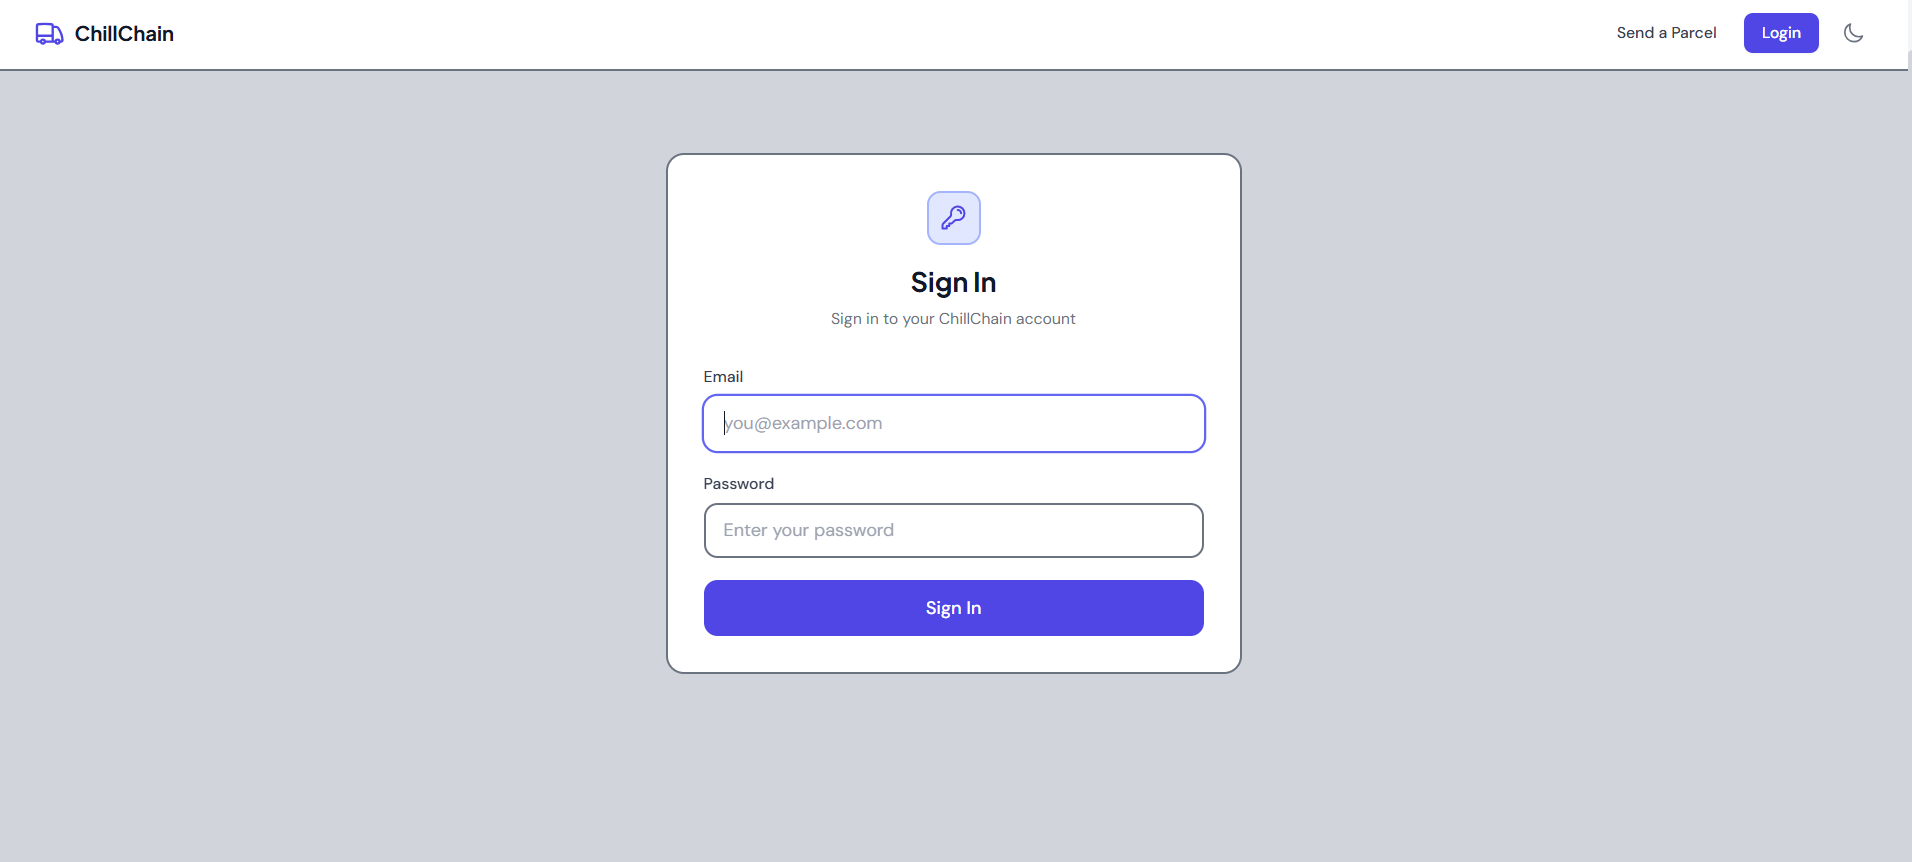
\includegraphics[width=0.95\textwidth]{img/val_login_admin.png}
\fbox{\parbox{0.9\textwidth}{\centering\vspace{3cm}\textit{Screenshot: schermata di login}\vspace{3cm}}}
\caption{Schermata di login della piattaforma. L'utente inserisce email e password; il sistema restituisce un token JWT e reindirizza alla dashboard corrispondente al ruolo.}
\label{fig:val_login}
\end{figure}

\begin{figure}[ht]
\centering
% 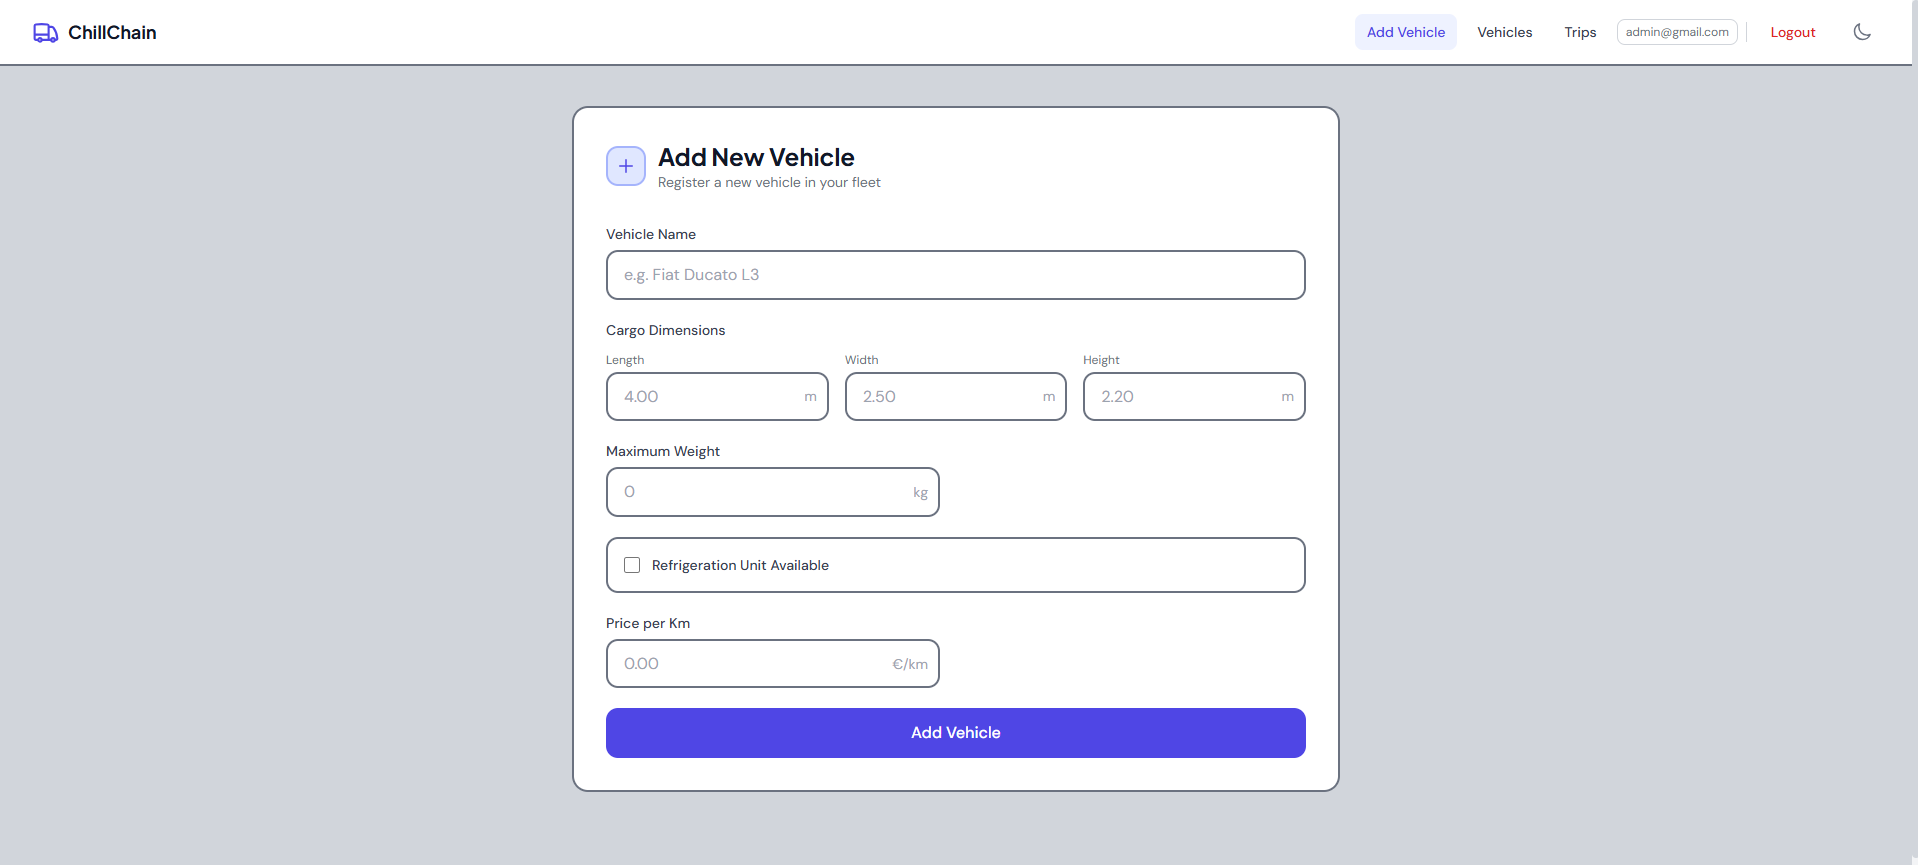
\includegraphics[width=0.95\textwidth]{img/val_add_vehicle.png}
\fbox{\parbox{0.9\textwidth}{\centering\vspace{3cm}\textit{Screenshot: form di aggiunta veicolo}\vspace{3cm}}}
\caption{Form di registrazione di un nuovo veicolo. L'amministratore specifica il nome identificativo, le dimensioni del vano di carico (larghezza, altezza, lunghezza in cm), il peso massimo trasportabile (kg), la tipologia di refrigerazione e il costo per chilometro (\euro/km).}
\label{fig:val_add_vehicle}
\end{figure}

Il primo veicolo, denominato \texttt{camion1}, è configurato con un vano di carico di 200\,$\times$\,200\,$\times$\,400~cm, peso massimo 1000~kg, refrigerazione attiva e costo di 0,50~\euro/km. Il secondo veicolo, \texttt{camion5}, ha dimensioni leggermente inferiori e un costo di 0,40~\euro/km. Entrambi i veicoli compaiono immediatamente nella lista della flotta.

\begin{figure}[ht]
\centering
% 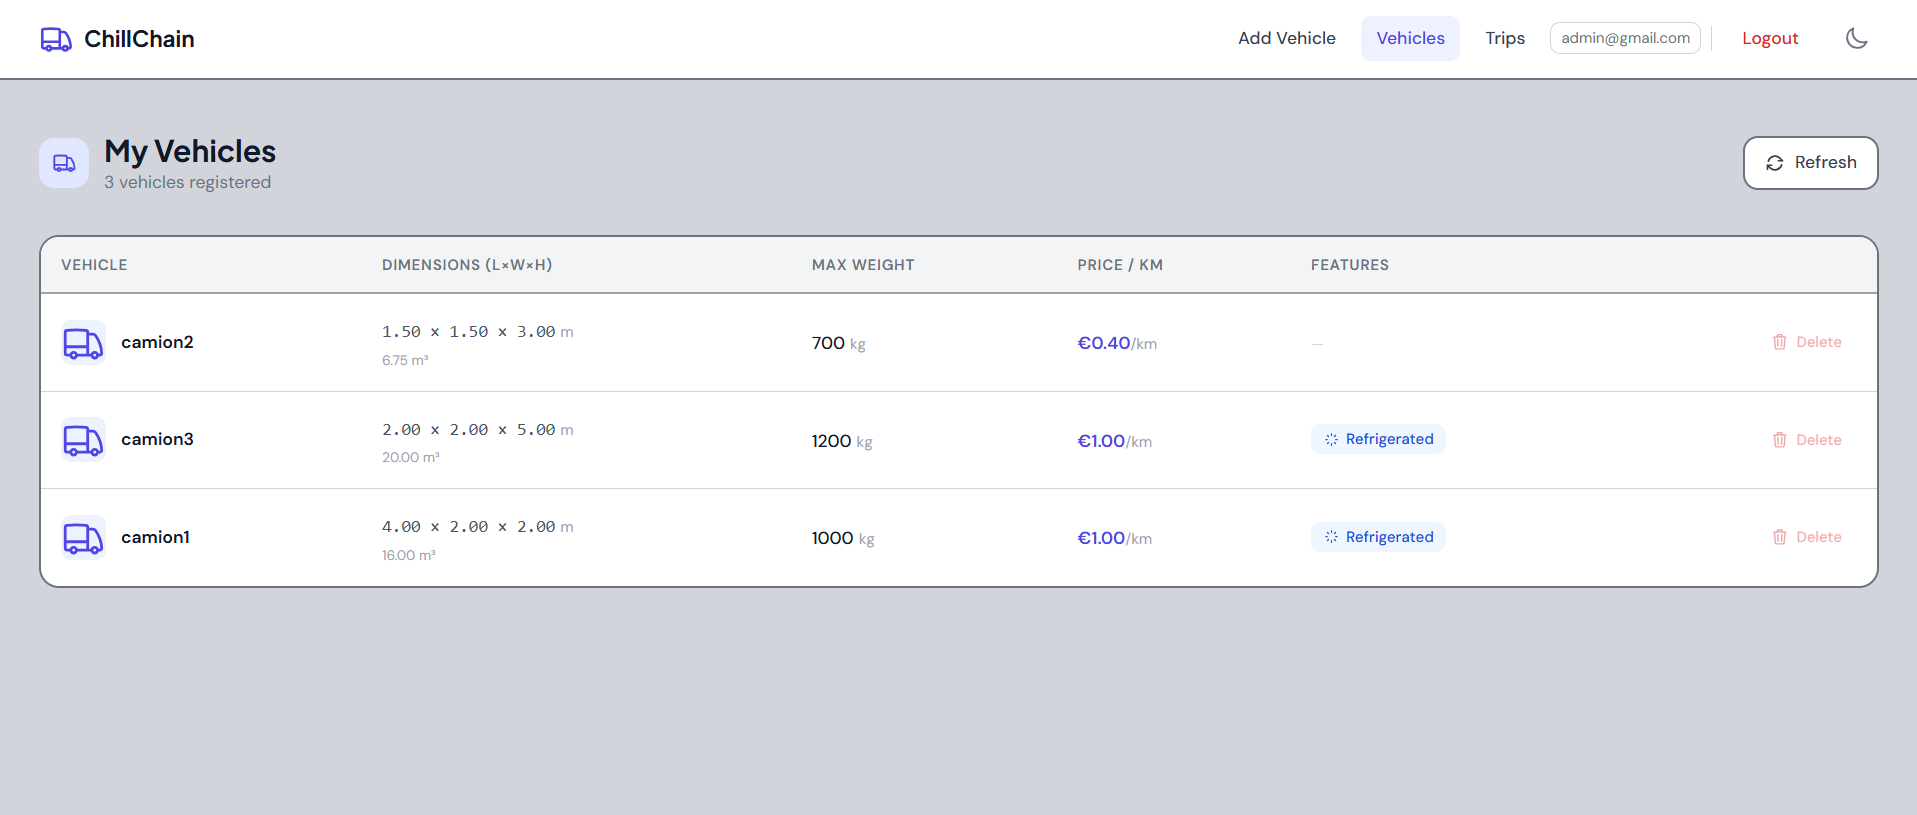
\includegraphics[width=0.95\textwidth]{img/val_vehicle_list.png}
\fbox{\parbox{0.9\textwidth}{\centering\vspace{3cm}\textit{Screenshot: lista veicoli della flotta}\vspace{3cm}}}
\caption{Lista dei veicoli registrati nella flotta. Per ciascun veicolo sono visualizzati il nome, le dimensioni, il peso massimo, lo stato di refrigerazione e il prezzo per chilometro. Le azioni disponibili includono l'eliminazione del veicolo e la visualizzazione delle tratte associate.}
\label{fig:val_vehicle_list}
\end{figure}


% ----------------------------------------------------------------------------
\subsection{Fase 2 --- Prima spedizione: creazione della tratta (Cliente A)}
\label{subsec:fase2}

Un primo cliente accede alla piattaforma e inserisce i dati della propria spedizione: partenza da Milano, arrivo a Roma, pacco di 50\,$\times$\,50\,$\times$\,50~cm con peso di 100~kg, refrigerazione necessaria e data di arrivo entro il 28 febbraio 2026.

\begin{figure}[ht]
\centering
% 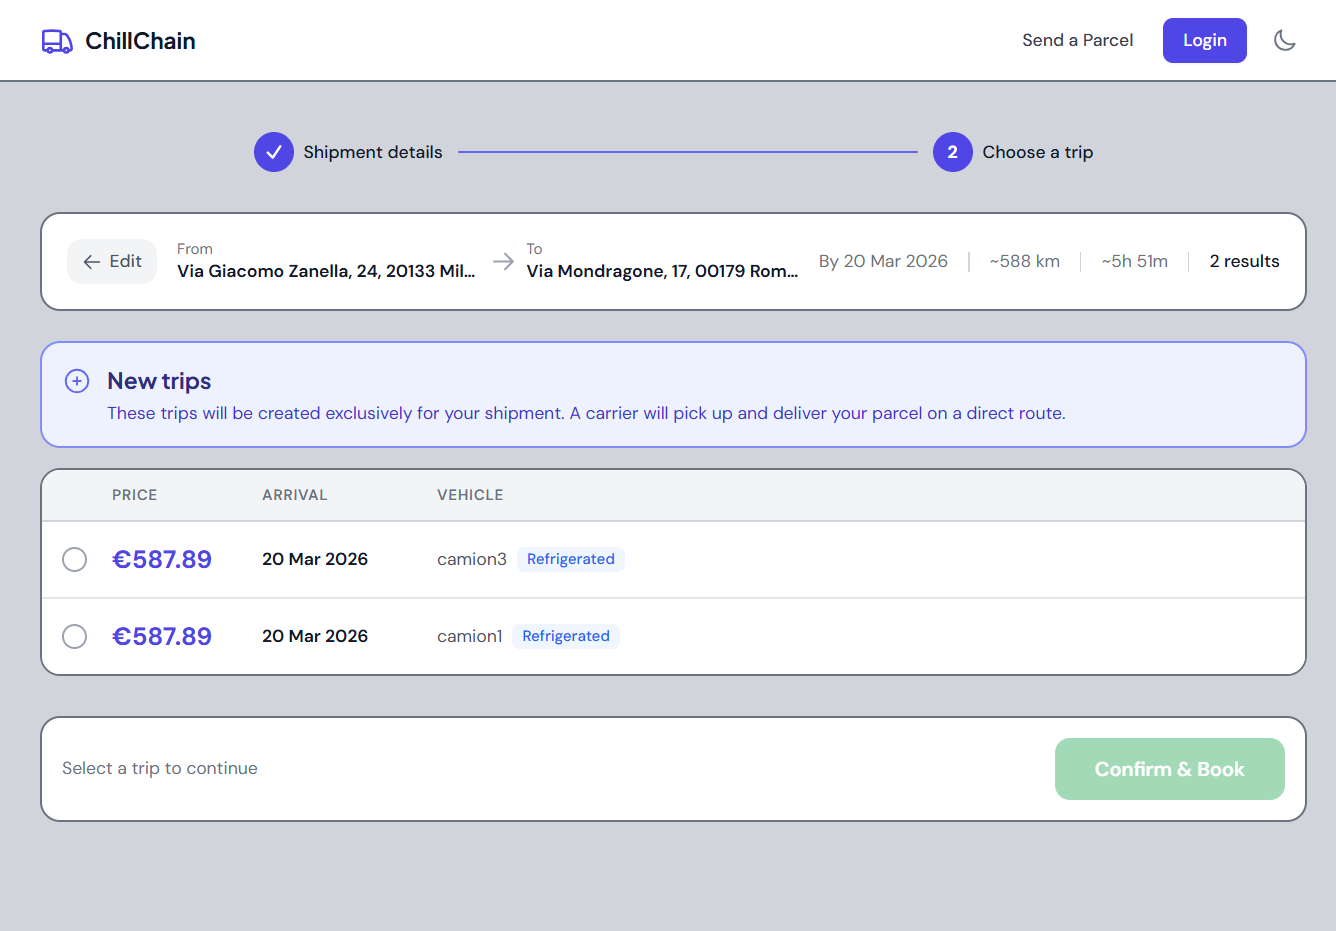
\includegraphics[width=0.95\textwidth]{img/val_send_parcel.png}
\fbox{\parbox{0.9\textwidth}{\centering\vspace{3cm}\textit{Screenshot: form di invio spedizione}\vspace{3cm}}}
\caption{Form di ricerca tratte. Il cliente inserisce gli indirizzi di partenza e arrivo, le dimensioni e il peso del pacco, la necessità di refrigerazione e la data di arrivo desiderata.}
\label{fig:val_send_parcel}
\end{figure}

Il sistema restituisce la lista delle tratte disponibili. In questo caso, poiché nessun veicolo ha ancora una tratta assegnata, vengono mostrati entrambi i veicoli come opzioni ``vuote'': \texttt{camion1} a 287,50~\euro{} e \texttt{camion5} a 230,00~\euro{} (calcolati come distanza Milano--Roma $\times$ prezzo/km del rispettivo veicolo). Per ciascuna opzione, il cliente può visualizzare il percorso su mappa prima di confermare.

\begin{figure}[ht]
\centering
% 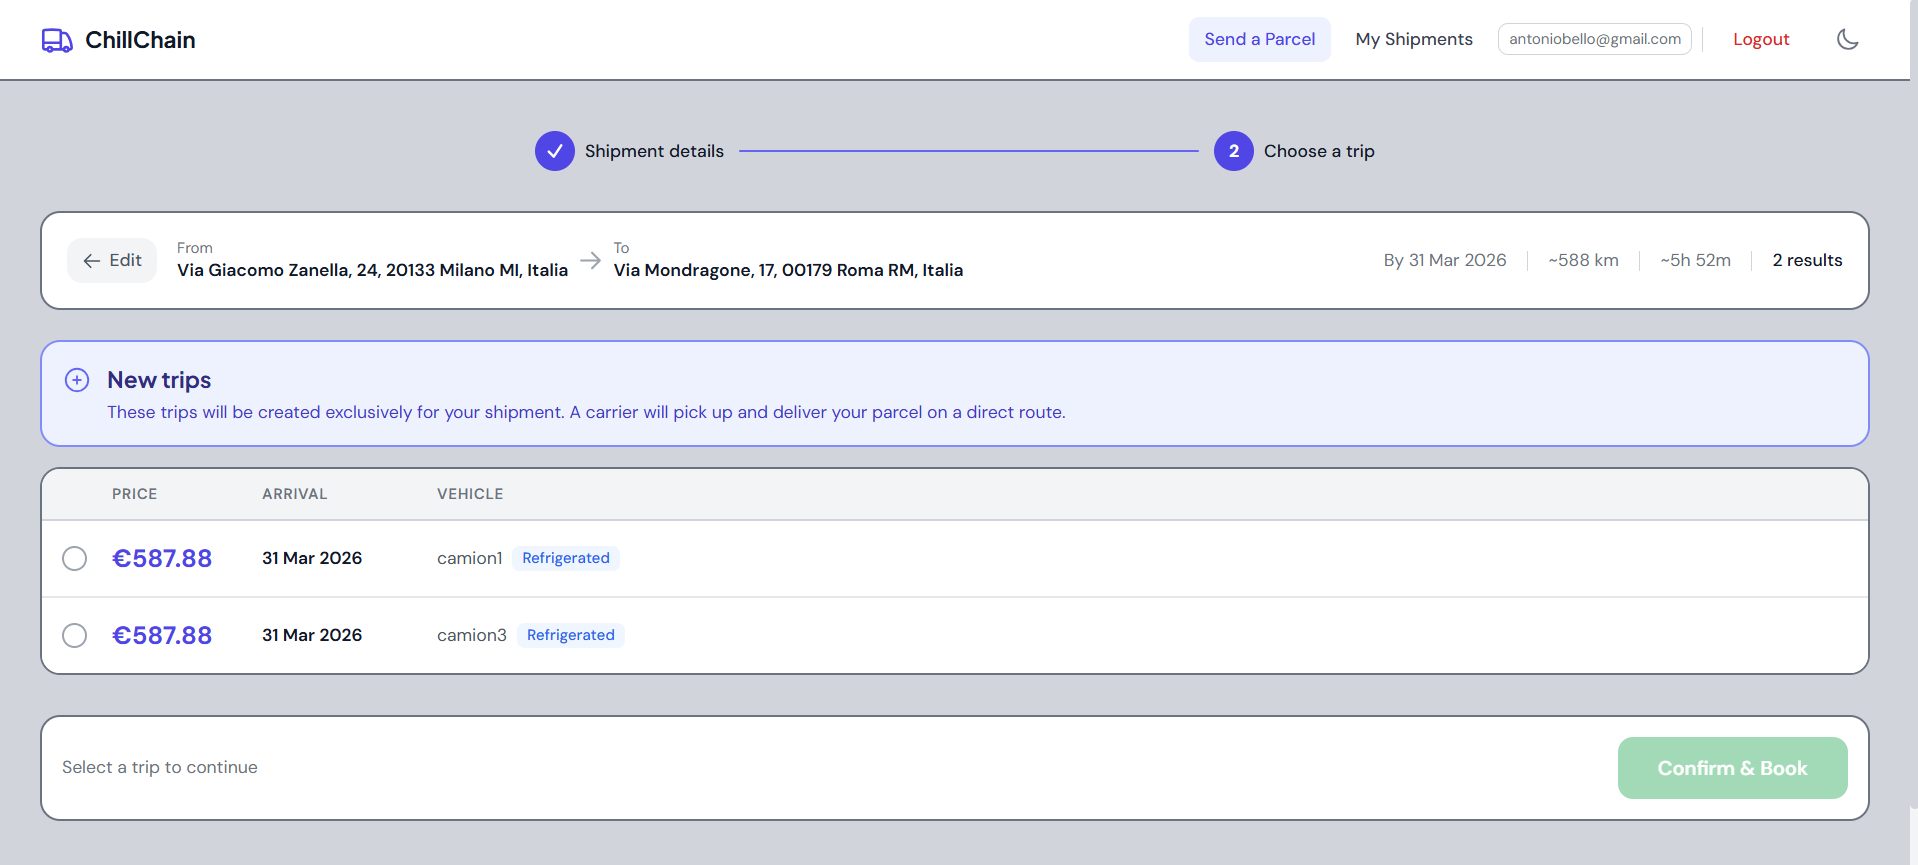
\includegraphics[width=0.95\textwidth]{img/val_trip_list_first.png}
\fbox{\parbox{0.9\textwidth}{\centering\vspace{3cm}\textit{Screenshot: lista tratte disponibili con mappa}\vspace{3cm}}}
\caption{Risultati della ricerca tratte per il Cliente A. Sono visibili due veicoli disponibili con il percorso Milano--Roma, prezzo calcolato, distanza e durata stimata. La mappa mostra la polyline del percorso selezionato.}
\label{fig:val_trip_list_first}
\end{figure}

Il Cliente A seleziona \texttt{camion1}. Il backend crea una nuova entità \texttt{Trip} con il percorso Milano--Roma, decrementa la capacità residua del veicolo e salva lo \texttt{Shipment} associato.


% ----------------------------------------------------------------------------
\subsection{Fase 3 --- Seconda spedizione: condivisione della tratta (Cliente B)}
\label{subsec:fase3}

Un secondo cliente effettua una ricerca per una spedizione da Bologna a Firenze, con un pacco più piccolo (30\,$\times$\,30\,$\times$\,30~cm, 20~kg, refrigerato, stesso periodo di arrivo).

\begin{figure}[ht]
\centering
% 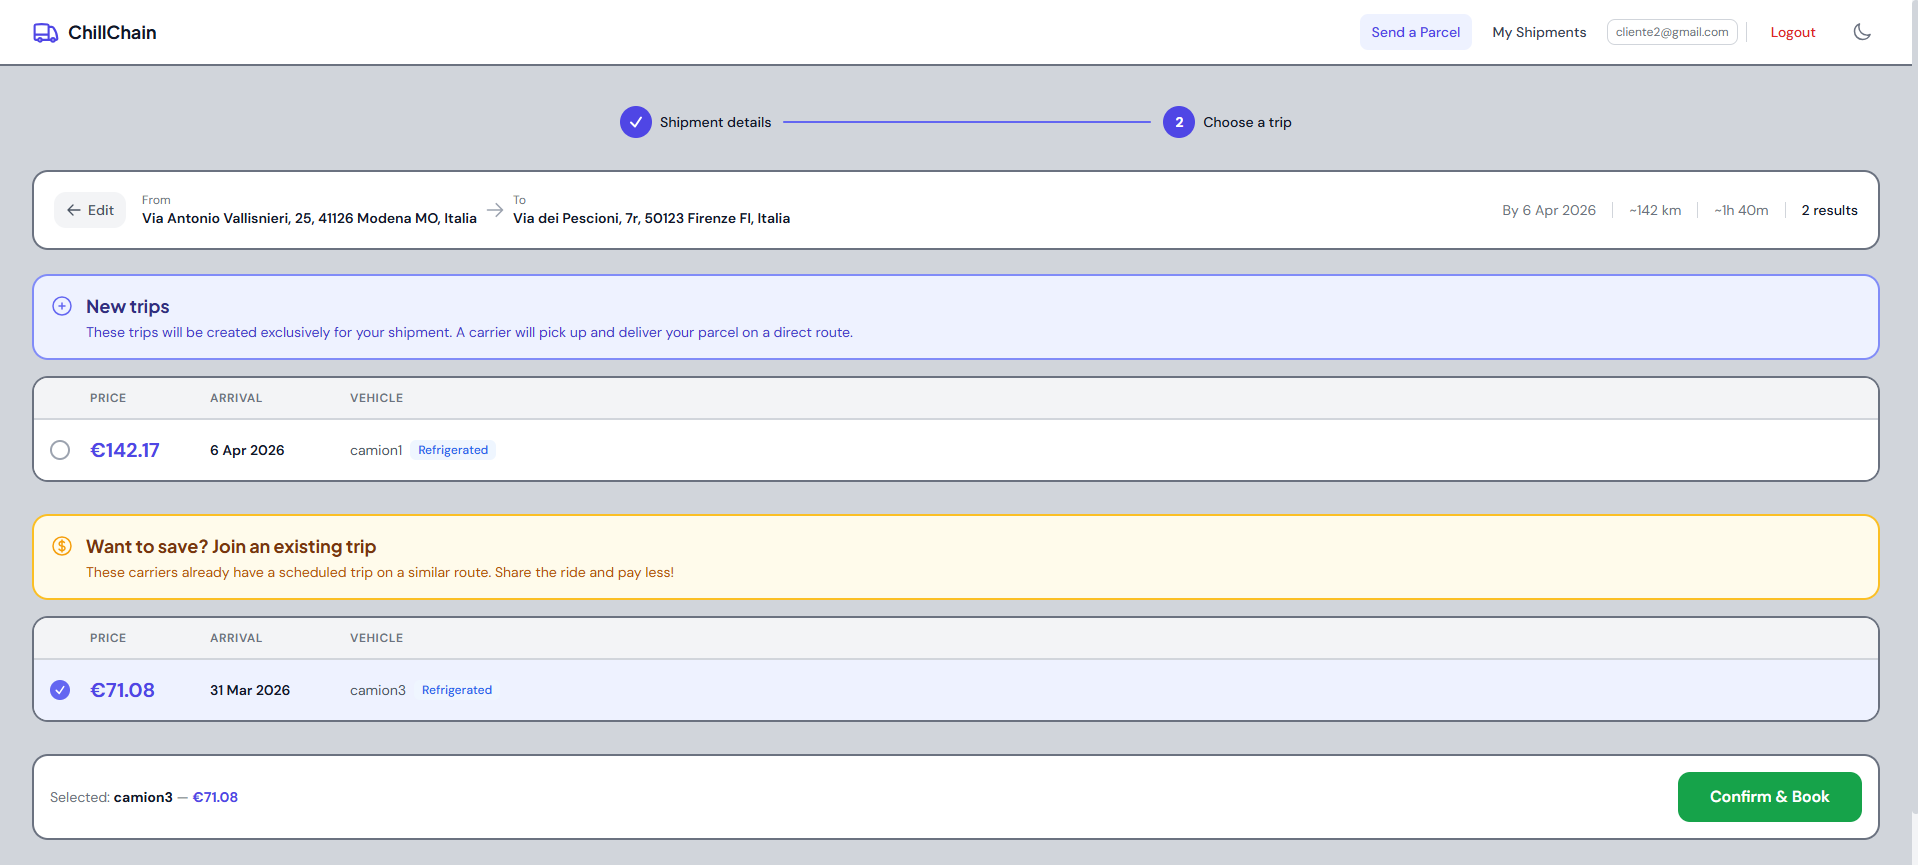
\includegraphics[width=0.95\textwidth]{img/val_trip_list_shared.png}
\fbox{\parbox{0.9\textwidth}{\centering\vspace{3cm}\textit{Screenshot: lista tratte con opzione condivisa}\vspace{3cm}}}
\caption{Risultati della ricerca tratte per il Cliente B. Oltre al veicolo \texttt{camion5} disponibile come tratta dedicata, compare \texttt{camion1} come tratta condivisa: il percorso Milano--Roma passa sufficientemente vicino a Bologna e Firenze, la deviazione rientra nei 30 minuti di tolleranza e il prezzo è scontato del 50\% grazie alla formula $2^n$ con $n=1$ spedizione già presente.}
\label{fig:val_trip_list_shared}
\end{figure}

Il sistema mostra tre opzioni: \texttt{camion5} come tratta dedicata (Bologna--Firenze a 46,00~\euro{}), \texttt{camion1} come tratta condivisa (il percorso ricalcolato Milano--Bologna--Firenze--Roma rientra nella tolleranza di 30 minuti, al prezzo scontato grazie al divisore $2^1$), e un'eventuale ulteriore opzione dedicata. Il Cliente B seleziona la tratta condivisa su \texttt{camion1}. Il backend aggiorna la polyline del trip con i nuovi waypoint (Bologna e Firenze come tappe intermedie), decrementa ulteriormente la capacità residua e salva il nuovo \texttt{Shipment}.


% ----------------------------------------------------------------------------
\subsection{Fase 4 --- Gestione della tratta e avvio simulazione (Amministratore)}
\label{subsec:fase4}

L'amministratore verifica che la tratta sia stata correttamente aggiornata, visualizzando nella sezione tratte il percorso ricalcolato con i waypoint intermedi e la lista delle spedizioni associate.

\begin{figure}[ht]
\centering
% 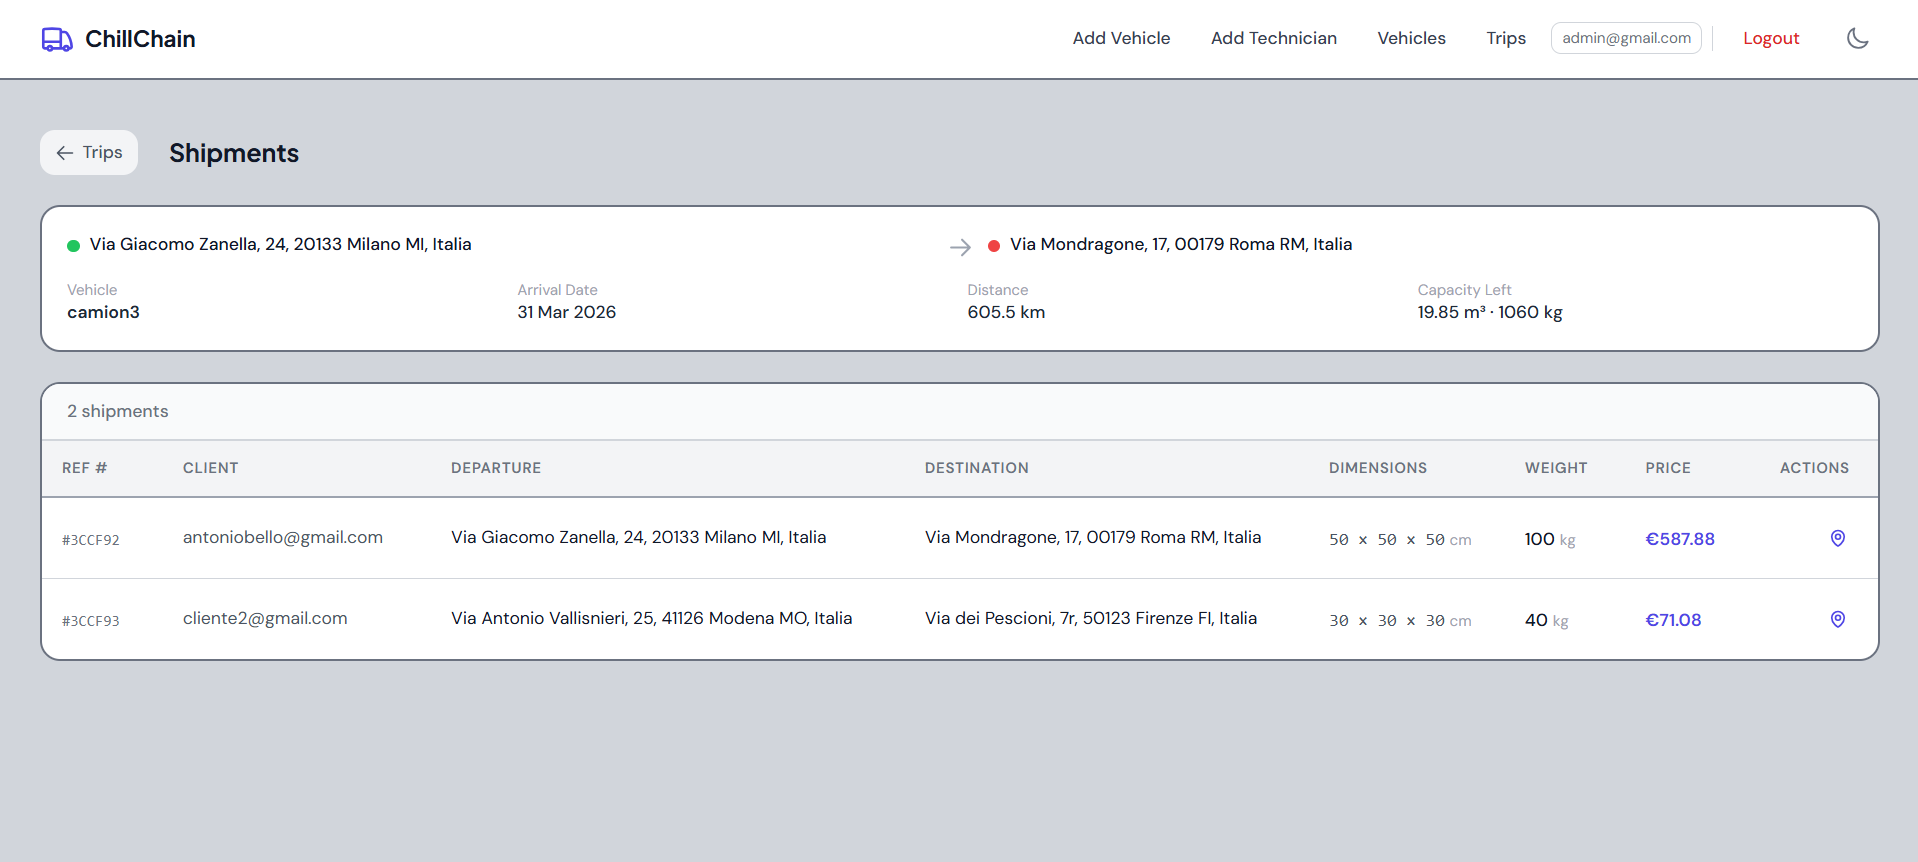
\includegraphics[width=0.95\textwidth]{img/val_trip_detail.png}
\fbox{\parbox{0.9\textwidth}{\centering\vspace{3cm}\textit{Screenshot: dettaglio tratta con spedizioni}\vspace{3cm}}}
\caption{Dettaglio della tratta assegnata a \texttt{camion1}, con il percorso aggiornato (Milano--Bologna--Firenze--Roma) e la lista delle due spedizioni associate. Sono visibili la distanza totale aggiornata, la durata e la capacità residua del veicolo.}
\label{fig:val_trip_detail}
\end{figure}

L'amministratore avvia quindi la simulazione della telemetria per \texttt{camion5}, associato al dataset contenente il guasto combinato. Il backend inoltra la richiesta al servizio di streaming, che inizia a pubblicare i dati sul topic \texttt{fridge/camion5/telemetry}.

\begin{figure}[ht]
\centering
% \includegraphics[width=0.95\textwidth]{img/val_start_simulation.png}
\fbox{\parbox{0.9\textwidth}{\centering\vspace{3cm}\textit{Screenshot: avvio simulazione telemetrica}\vspace{3cm}}}
\caption{Avvio della simulazione telemetrica per il veicolo \texttt{camion5}. Il pulsante ``Start Simulation'' attiva lo streaming dei dati dal CSV al broker MQTT. Lo stato della simulazione mostra il progresso (riga corrente/totale).}
\label{fig:val_start_simulation}
\end{figure}


% ----------------------------------------------------------------------------
\subsection{Fase 5 --- Rilevazione anomalia e notifica (Tecnico)}
\label{subsec:fase5}

Il tecnico accede alla piattaforma con le proprie credenziali e viene indirizzato alla dashboard di monitoraggio. Durante i primi 60 minuti simulati, il modello LSTM Autoencoder ricostruisce correttamente le sequenze: l'errore di ricostruzione oscilla intorno a valori di 0,005--0,008, ben al di sotto della soglia configurata.

\begin{figure}[ht]
\centering
% \includegraphics[width=0.95\textwidth]{img/val_telemetry_normal.png}
\fbox{\parbox{0.9\textwidth}{\centering\vspace{3cm}\textit{Screenshot: dashboard telemetrica in condizioni normali}\vspace{3cm}}}
\caption{Dashboard telemetrica del veicolo \texttt{camion5} durante la fase di funzionamento normale (primi 60 minuti). I grafici mostrano i parametri operativi dell'impianto frigorifero: la temperatura della cella ($T_{\text{cab\_meas}}$) oscilla intorno al setpoint, il COP è stabile e le pressioni sono nel range atteso.}
\label{fig:val_telemetry_normal}
\end{figure}

A partire dal minuto 60, il dataset inietta il guasto \texttt{UNDERCHARGE\_AND\_COND\_FOUL}: il sottocaricamento del refrigerante causa un aumento del surriscaldamento e una riduzione della capacità frigorifera, mentre il fouling del condensatore innalza la temperatura e la pressione di condensazione. Il modello inizia a produrre errori di ricostruzione superiori alla soglia. Dopo 20 campioni consecutivi anomali (il meccanismo di smoothing), il servizio di anomaly detection pubblica un messaggio di allerta sul topic \texttt{fridge/camion5/anomalies}.

Il backend riceve il messaggio, crea una notifica persistente e la rende disponibile al tecnico. L'icona delle notifiche nell'header si aggiorna con il badge numerico.

\begin{figure}[ht]
\centering
% 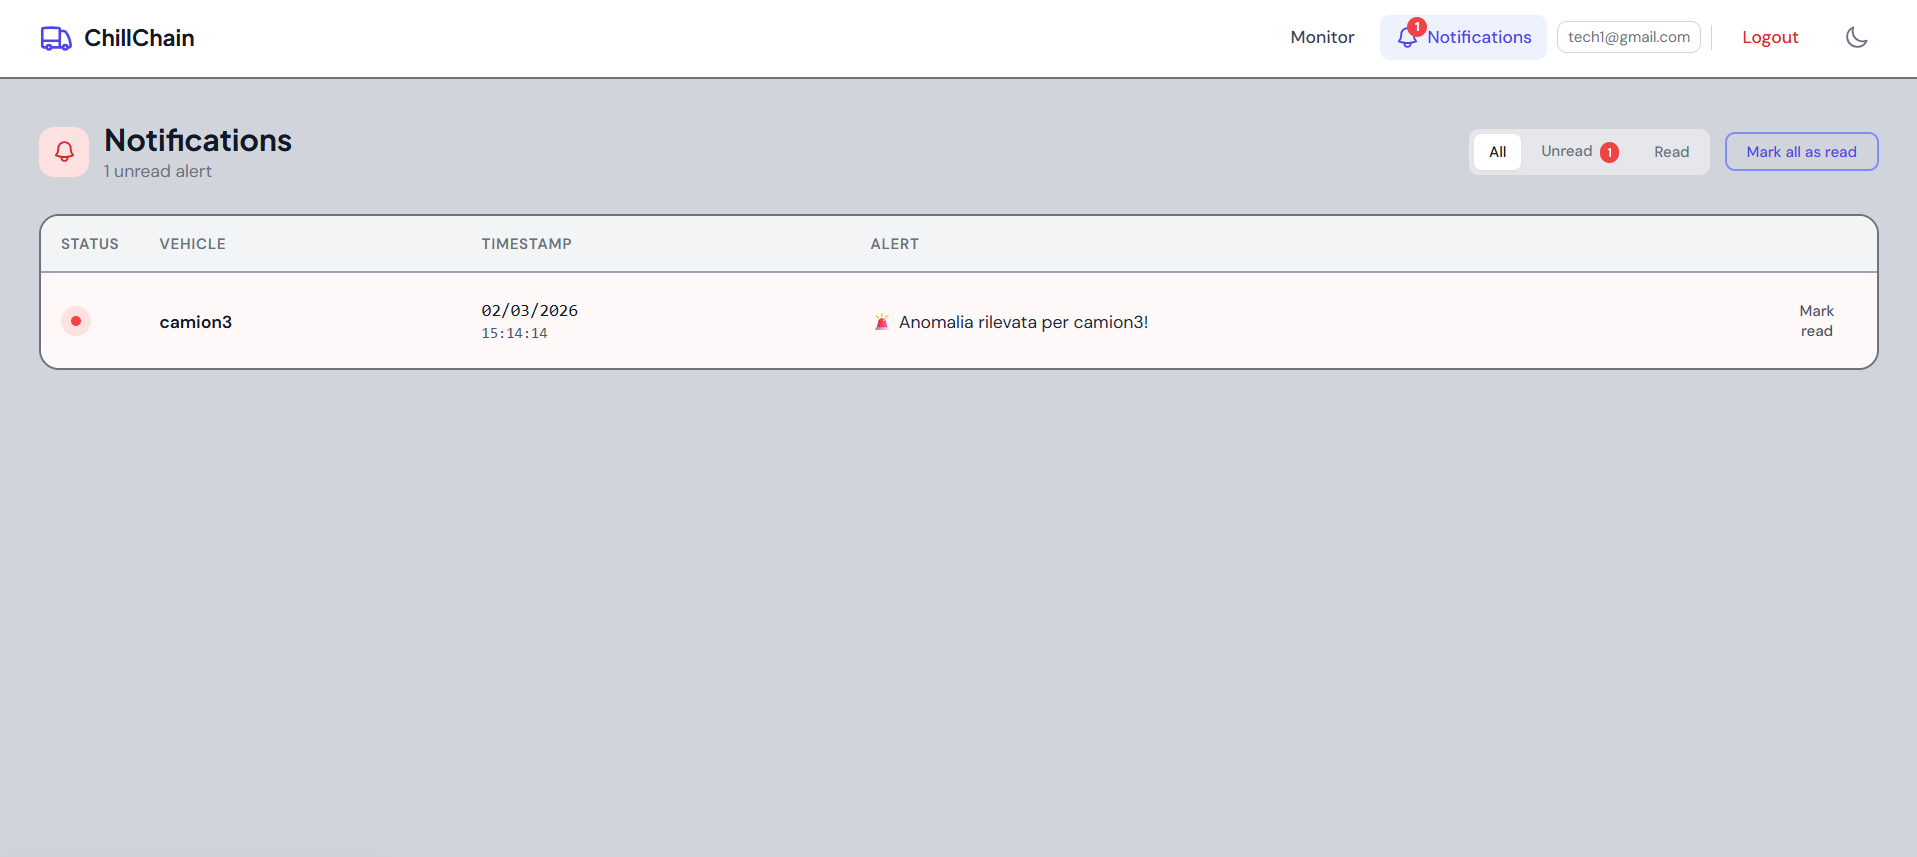
\includegraphics[width=0.95\textwidth]{img/val_notification.png}
\fbox{\parbox{0.9\textwidth}{\centering\vspace{3cm}\textit{Screenshot: notifica di anomalia ricevuta}\vspace{3cm}}}
\caption{Pannello notifiche del tecnico. La notifica indica il veicolo interessato (\texttt{camion5}), il timestamp dell'allerta, l'errore di ricostruzione e il messaggio ``Anomalia rilevata per camion5!''. Il badge nell'header mostra il conteggio delle notifiche non lette.}
\label{fig:val_notification}
\end{figure}

Il tecnico seleziona la notifica e accede alla dashboard telemetrica di \texttt{camion5}. I grafici mostrano chiaramente la transizione: intorno al campione 60, la temperatura della cella inizia a salire, il COP diminuisce, la pressione di scarico aumenta e il surriscaldamento cresce sensibilmente.

\begin{figure}[ht]
\centering
% 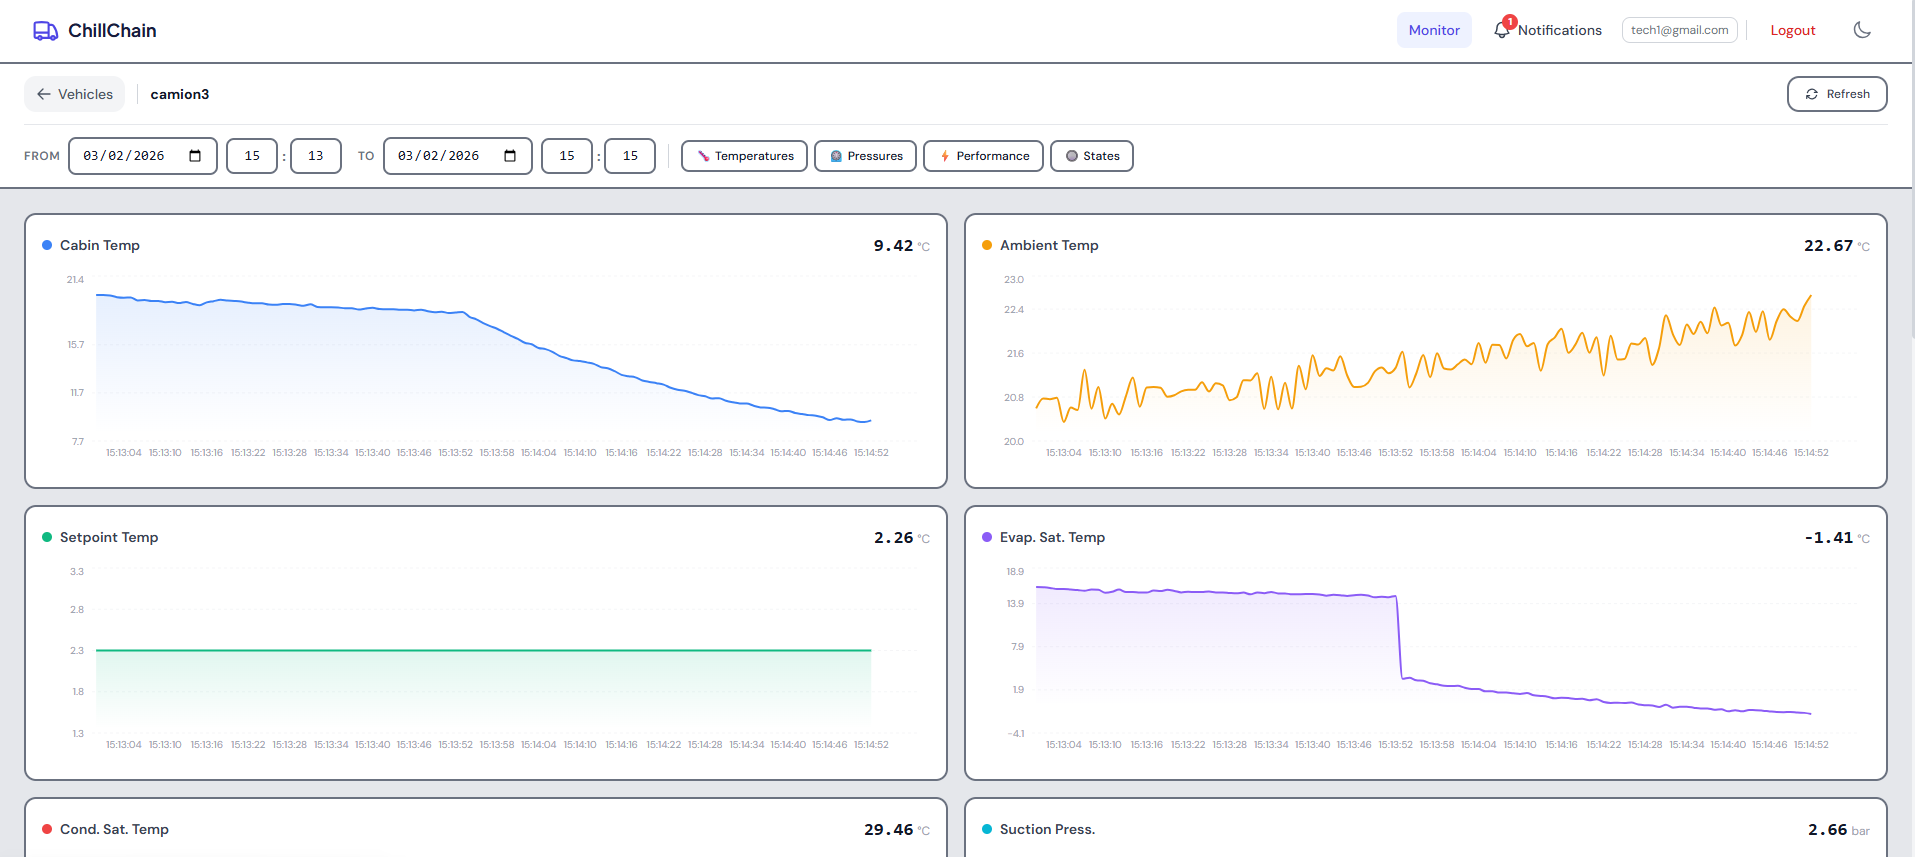
\includegraphics[width=0.95\textwidth]{img/val_telemetry_anomaly.png}
\fbox{\parbox{0.9\textwidth}{\centering\vspace{3cm}\textit{Screenshot: dashboard telemetrica con anomalia visibile}\vspace{3cm}}}
\caption{Dashboard telemetrica del veicolo \texttt{camion5} dopo l'iniezione del guasto. A partire dal campione 60, i grafici evidenziano il degrado delle prestazioni: innalzamento di $T_{\text{cab\_meas}}$ e $T_{\text{cond\_sat}}$, aumento di $P_{\text{dis\_bar}}$ e $SH_K$, riduzione del COP. La codifica cromatica passa dal verde al rosso nella zona anomala.}
\label{fig:val_telemetry_anomaly}
\end{figure}


% ============================================================================
\section{Esito della validazione}
\label{sec:esito}

Lo scenario descritto ha permesso di verificare il corretto funzionamento di tutte le funzionalità della piattaforma lungo l'intero flusso operativo.

Per quanto riguarda il marketplace, la registrazione dei veicoli, la ricerca delle tratte con filtro dimensionale e temporale, il ricalcolo del percorso con waypoint e il pricing con divisore esponenziale hanno prodotto risultati coerenti con le attese: il prezzo della tratta condivisa è risultato effettivamente dimezzato rispetto a quello della tratta dedicata, e la polyline aggiornata ha incluso correttamente le tappe intermedie di Bologna e Firenze.

Sul versante del monitoraggio, il modello LSTM Autoencoder ha ricostruito correttamente le sequenze normali (errore sotto soglia per i primi 60 minuti) e ha rilevato il degrado delle prestazioni a partire dal minuto 60. Il meccanismo di smoothing ha evitato falsi positivi durante la fase normale e ha generato la notifica circa 20 minuti dopo l'inizio del guasto, in linea con il comportamento atteso del contatore a 20 campioni consecutivi. La notifica è stata correttamente persistita su MongoDB e resa disponibile al tecnico, che ha potuto analizzare lo storico dei dati e identificare visivamente la transizione nei grafici telemetrici.

La comunicazione tra i servizi si è dimostrata affidabile: i messaggi MQTT sono stati instradati correttamente dallo streamer all'anomaly detector e da quest'ultimo al backend, senza perdita di dati osservabile. L'avvio e l'arresto della simulazione dal frontend hanno funzionato come previsto, con il messaggio di completamento che ha attivato la pulizia delle risorse del detector.

La separazione delle viste per ruolo ha operato correttamente: l'amministratore ha avuto accesso esclusivamente alla gestione della flotta e delle tratte, il cliente alla ricerca e prenotazione, il tecnico al monitoraggio e alle notifiche. Tentativi di accesso a endpoint non autorizzati hanno restituito correttamente l'errore HTTP 403.